%
% compile with pdflatex:
%   $ pdflatex homework-hw
% , yields homework-example.pdf
%    You might need to compile twice, if, e.g., you start using references
%

\documentclass[10pt,letterpaper,oneside]{article}
\usepackage[ascii]{inputenc}
\usepackage{graphicx}
\graphicspath{ {} }
\usepackage{amsmath,amsfonts,amssymb}
\usepackage[margin=1in]{geometry}
	\setlength{\parindent}{0em}
	\setlength{\parskip}{1em}



\newtheorem{theorem}{Theorem}

%%%% user definitions %%%%%%%%%%%%%%%%%%%%%%%

\newcommand{\Problem}[1]{\subsection*{Problem #1}}
\newcommand{\Part}[1]{\subsubsection*{Part #1}}
\newcommand{\Solution}{\subsubsection*{Solution}}

	% Forms for Big-Oh notation
\DeclareMathOperator{\Omicron}{O}
\DeclareMathOperator{\omicron}{o}

\newcommand{\BigOh}[1]{\Omicron(#1)}
\newcommand{\LittleOh}[1]{\omicron(#1)}
\newcommand{\BigOmega}[1]{\Omega(#1)}
\newcommand{\LittleOmega}[1]{\omega(#1)}
\newcommand{\BigTheta}[1]{\Theta(#1)}

	% Operators for dominance notation
\newcommand{\domeq}{\sim}
\newcommand{\domle}{\preceq}
\newcommand{\domlt}{\prec}
\newcommand{\domge}{\succeq}
\newcommand{\domgt}{\succ}

\newcommand\tab[1][1cm]{\hspace*{#1}}


%%%%%%%%  You edit stuff below this line  %%%%%%%%%%%%%%%%%%%%%%%%%%

\title{HW3 Theory}
\author{Alexander Kazantsev}
%\date{}  % uses today, by default

\begin{document}

\maketitle

\Problem{1}

\textbf{Fib-Normal}

def fib(n):

	\tab if n $<$ 2:

	\tab\tab	return 1

	\tab return fib(n-1) + fib(n-2)

\textbf{Fib-Memo}

memoSize = 100

memo = [None] * memoSize 

def FibMemo(n):

	\tab global memo

	\tab memo = [None] * memoSize

	\tab return FibMemoAlgo(n)


def FibMemoAlgo(n):

	\tab if memo[n] != None:

		\tab\tab return memo[n]

	\tab if n $<=$ 1:

	\tab\tab	return 1

	\tab val = FibMemoAlgo(n-1) + FibMemoAlgo(n-2)

	\tab memo[n] = val

	\tab return val

The time complexity of the normal Fibonacci algorithm is $\BigOh{2^n}$. This is because it forms a binary tree, and at minimum will have a height of $n-1$ from the root of the tree, therefore it will have on average $2^n$ nodes. 

The time complexity of the memoization Fibonacci algorithm is $\BigOh{n}$, or linear. The reason it is linear and more efficient than the standard Fibonacci algorithm is because it doesn't have to visit each node in the tree. The Fiboncci algorithm visits nodes in postfix form (Left Right Current), which means the most left branch will be generated "first". One branch is usually generated in linear time. Once the left most branch is generated, all of the Fibonacci values are available from $[0,n-1]$ and must only be added up with each left most nodes right sibling, which again is linear time. This is a significantly faster algorithm, even without permanent storage.    

\Problem{2}
If the size of the memo list was unbounded, the time complexity would still be linear. If memo list is of current size $m$ and an input of $n$ was given where $n>m$, also assuming $n$ is os significant size larger, then the memo list would have to grow by a size of $n-m$ once. Since $n-m \in \BigOh{n}$ the operation is linear, and since it is performed only once the rules of additivity can be envoked. The algorithm is still linear.

\Problem{3.1}

\Part{a}
\tab All the nodes are leaves
\Part{b}
\tab $A$ is the root
\Part{c}
\tab $A$ is the parent node of $C$
\Part{d}
\tab $F$, $G$, and $H$ are children of $C$
\Part{e}
\tab $B$ and $A$ are ancestors of $E$
\Part{f}
\tab $I$, $M$, and $N$ are decendants of $E$
\Part{g}
\tab $E$ is $D$'s right sibling, but $E$ has no right sibling
\Part{h}
$J$ and $K$
\Part{i}
$C$ has a depth of 2
\Part{j}
$C$ has a height of 2
\Problem{3.2}
6 paths with a length of 3
\Problem{3.6}
\begin{tabular}{ |p{3cm}||p{3cm}|p{3cm}|p{3cm}|  }
 \hline

 \hline
 &pre($n$) $<$ pre($m$) & in($n$) $<$ in($m$)& post($n$) $<$ post($m$)\\
 \hline
 $n$ left of $m$   &    &\checkmark &\checkmark  \\
 $n$ right of $m$ &     &\checkmark    &\checkmark\\
 $n$ ancestor $m$ &\checkmark &\checkmark &  \\
 $n$ decendant $m$    & & \checkmark& \checkmark \\
 
 \hline
\end{tabular}

\Problem{3.20}

           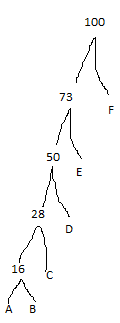
\includegraphics{tree.png}   

$1$ is left $0$ is right

A: 11111
B: 11110
C: 1110
D: 110
E: 10
F: 0

Average bits = .27 + 2*.23 + 3*.22 + 4* .12 + 5* .09 + 6* .07 = 2.74 bits/letter

\Problem{3.21}
Math and stuff like that... It's 3 AM and I'm tired, and this is a star problem
\end{document}

